\documentclass[aspectratio=169]{beamer}

\usetheme{Madrid}
\usecolortheme{seahorse}
\setbeamertemplate{navigation symbols}{}
\setbeamertemplate{footline}[frame number]

\usepackage{graphicx}
\usepackage{booktabs}
\usepackage{array}
\usepackage{amsmath}

\graphicspath{{../Figures/}}

\title{Deep Learning-Based Animal Re-Identification\\for Non-Invasive Wildlife Monitoring and Conservation}
\subtitle{MSc Thesis Defense (15 min)}
\author{Matej Mari\'c}
\institute{University of Zagreb\\Faculty of Electrical Engineering and Computing}
\date{February 2026}

\begin{document}

\begin{frame}[plain]
  \titlepage
\end{frame}

\begin{frame}{Motivation: Why a Species-Agnostic Pipeline?}
  \begin{columns}[T,totalwidth=\textwidth]
    \begin{column}{0.44\textwidth}
      \Large
      \begin{itemize}
        \item Unified pipeline across species
        \item Minimal supervision, practical runtime
        \item Re-ID as a building block for counting
      \end{itemize}
    \end{column}
    \begin{column}{0.54\textwidth}
      \centering
      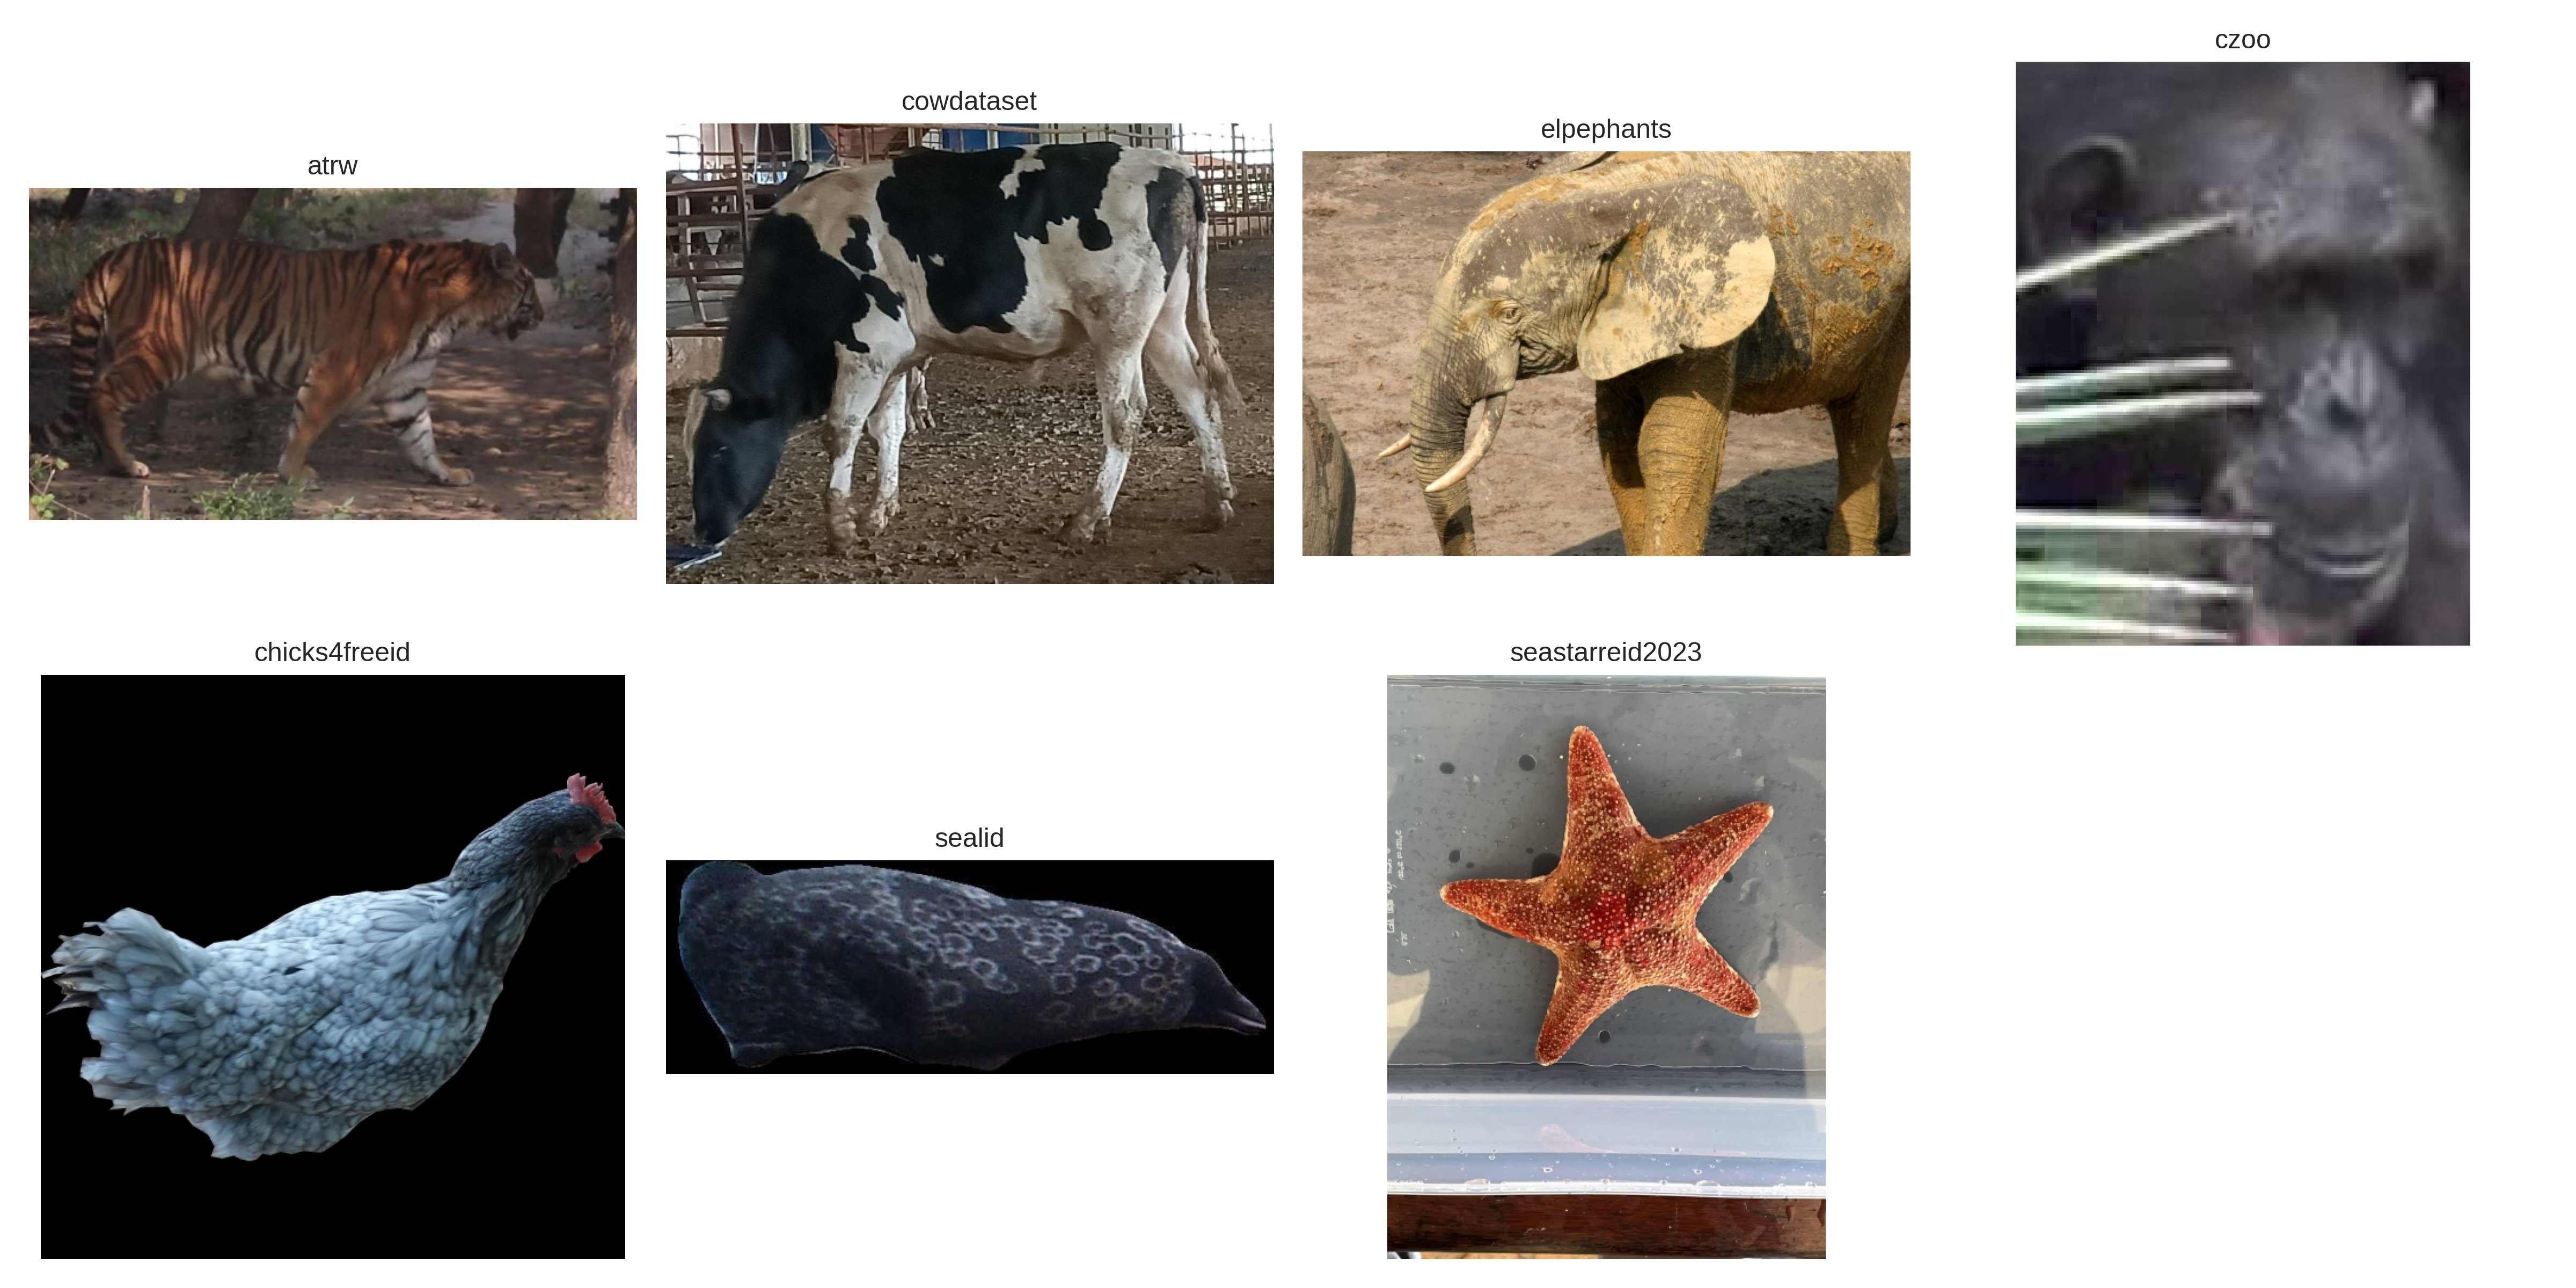
\includegraphics[width=\linewidth,height=0.80\textheight,keepaspectratio]{dataset_examples_grid.JPG}
    \end{column}
  \end{columns}
\end{frame}

\begin{frame}{Datasets: WildlifeReID-10k (7 Used Here)}
  \Large
  \begin{itemize}
    \item WildlifeReID-10k aggregates 37 datasets (33 species, 140k images, 10.7k individuals)
    \item Evaluated on 7 datasets spanning easy to hard cases (closed-set protocol)
  \end{itemize}

  \vspace{0.20cm}
  \centering
  \small
  \setlength{\tabcolsep}{5pt}
  \renewcommand{\arraystretch}{1.10}
  \begin{tabular}{l r r l}
    \toprule
    \textbf{Dataset} & \textbf{\# images} & \textbf{\# individuals} & \textbf{split type}\\
    \midrule
    ATRW* & 5,415 & 182 & Original MD split \\
    CZoo* & 4,662 & 71 & Original MD split \\
    SealID* & 2,080 & 57 & Original MD split \\
    CowDataset & 1,485 & 13 & Time-aware split \\
    Chicks4FreeID & 1,146 & 50 & Similarity-aware split \\
    SeaStarReID2023 & 2,187 & 95 & Time-aware split \\
    ELPephants & 2,078 & 276 & Random split \\
    \bottomrule
  \end{tabular}

  \vspace{0.10cm}
  \footnotesize
  * MD-trained datasets: use the exact training split to avoid additional leakage.
\end{frame}

\begin{frame}{Evaluation Rigor: Leakage Control}
  \begin{columns}[T,totalwidth=\textwidth]
    \begin{column}{0.52\textwidth}
      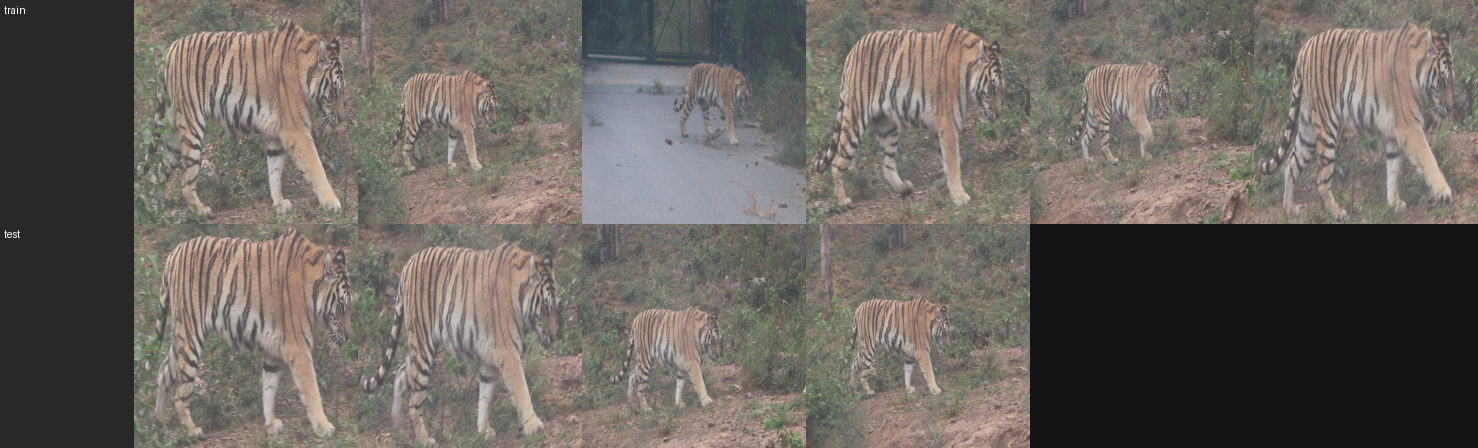
\includegraphics[width=\linewidth,height=0.72\textheight,keepaspectratio]{atrw_data_leak.png}
    \end{column}
    \begin{column}{0.46\textwidth}
      \vspace{0.04\textheight}
      \Large
      \begin{itemize}
        \item Time-aware splits
        \item Similarity-aware splits
        \item MD-train split alignment (ATRW/CZoo/SealID)
      \end{itemize}
    \end{column}
  \end{columns}
\end{frame}

\begin{frame}{Classification Funnel: Retrieve \textrightarrow\ Rerank \textrightarrow\ Verify}
  \Large
  \begin{itemize}
    \item Tier-1: retrieve candidates (Global + Fisher) and take the union
    \item Tier-2: calibrate and fuse scores into same-ID probability
    \item Tier-3: geometric verification (keypoints + RANSAC) on the shortlist
  \end{itemize}
\end{frame}

\begin{frame}{Pipeline Overview (Full)}
  \centering
  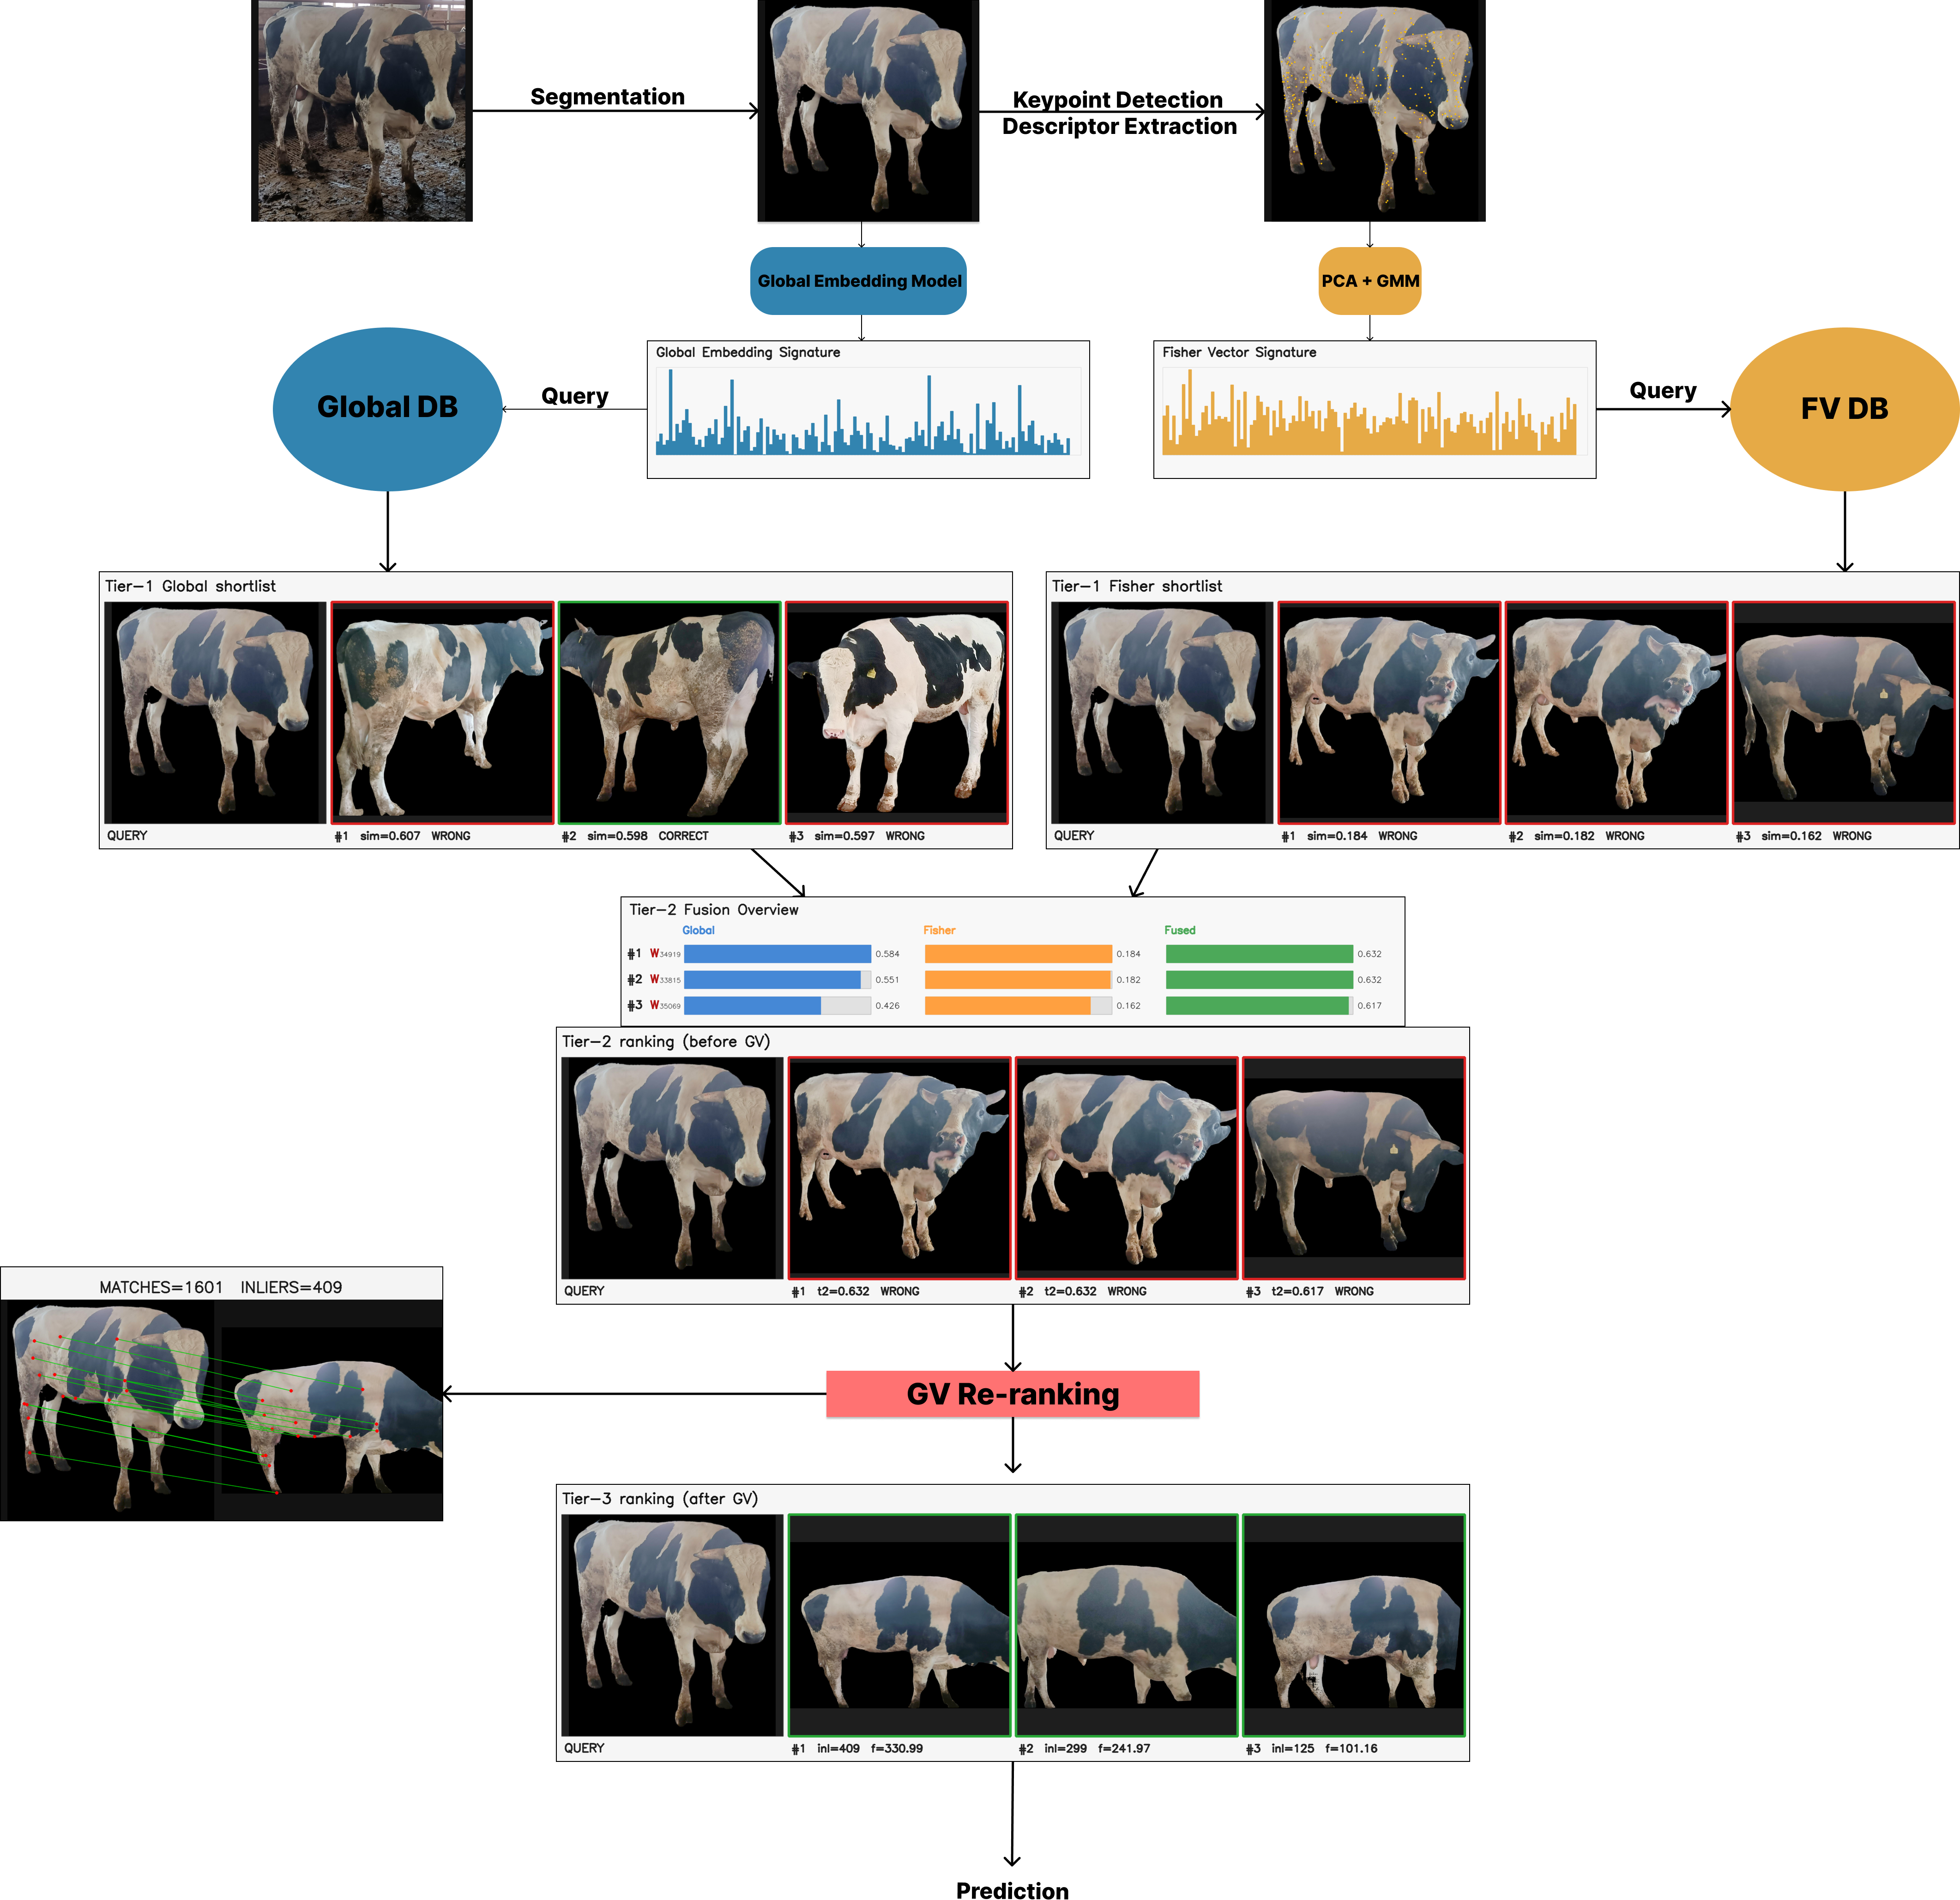
\includegraphics[width=0.98\linewidth,height=0.82\textheight,keepaspectratio]{classification_pipeline.png}
\end{frame}

\begin{frame}{Tier 1: Candidate Retrieval (Concept)}
  \Large
  \begin{itemize}
    \item Two fast signals: Global embeddings + Fisher vectors
    \item Take top-$K$ from each and form an ordered union (deduped)
    \item Goal: high-recall shortlist for expensive stages
    \item Background removal helps stabilize local evidence (optional)
  \end{itemize}
\end{frame}

\begin{frame}{Tier 1: Candidate Retrieval (Visualization)}
  \centering
  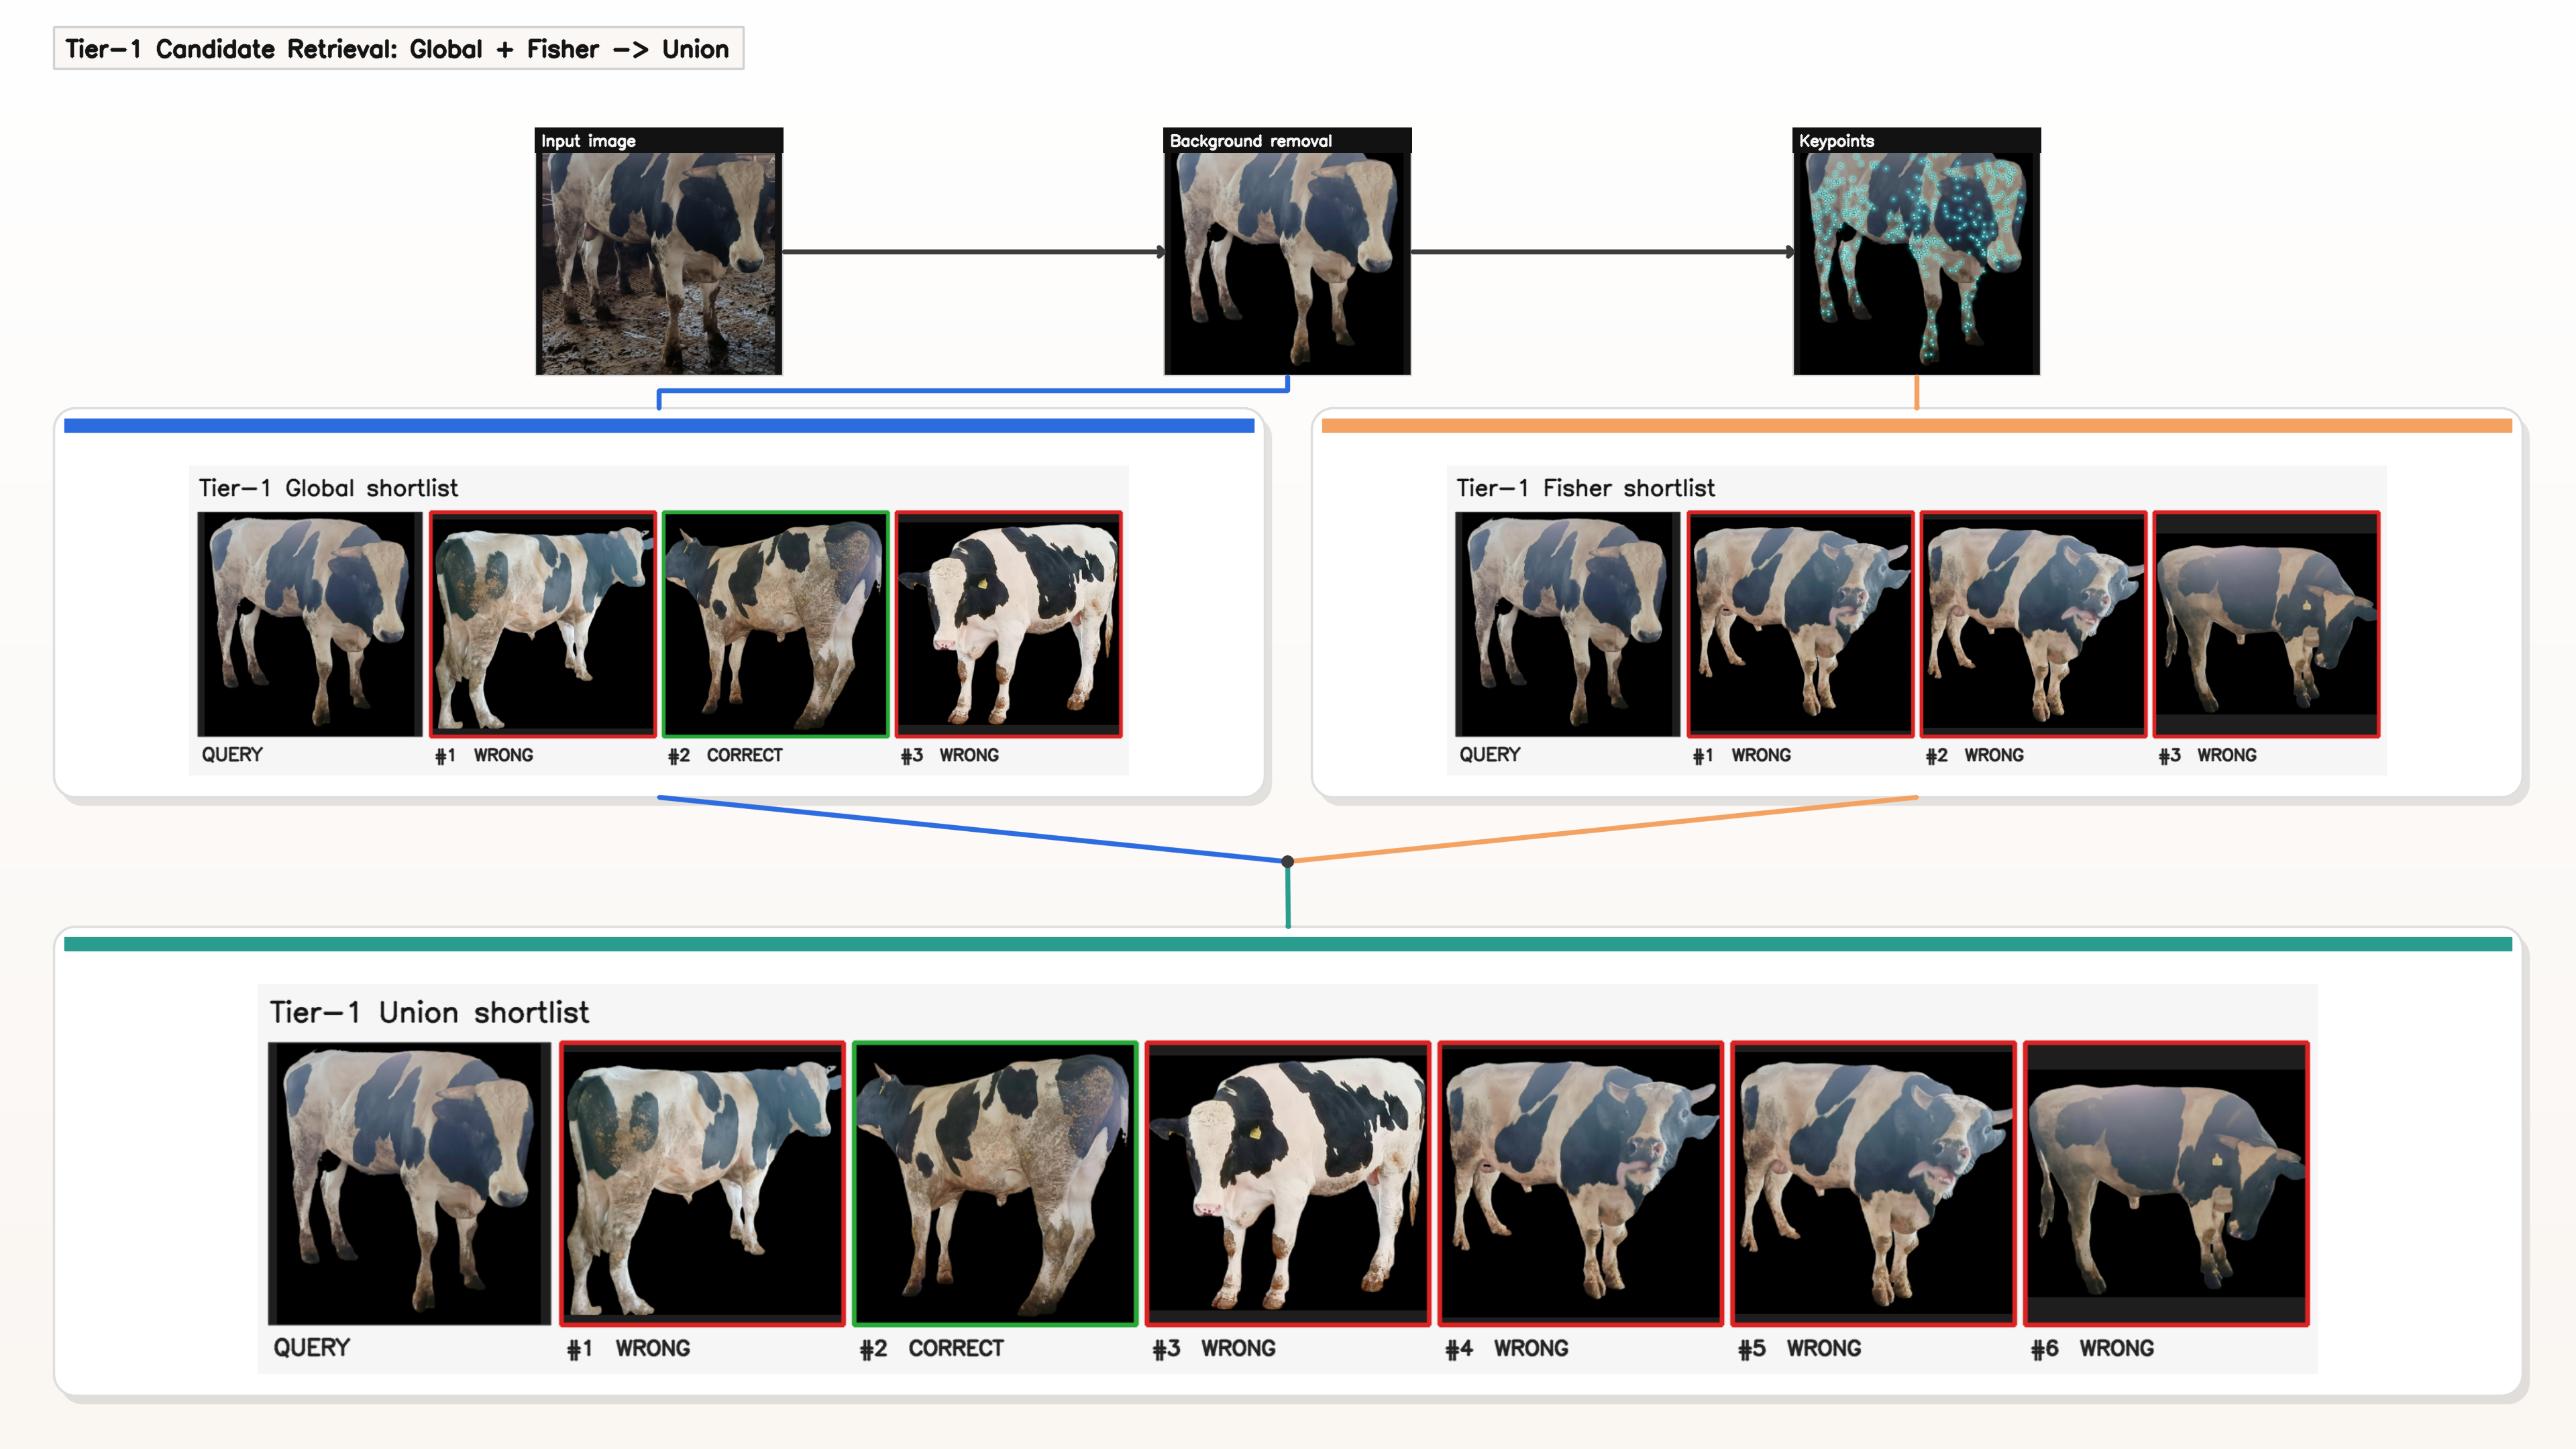
\includegraphics[width=0.98\linewidth,height=0.82\textheight,keepaspectratio]{tier1_union_flow.png}
\end{frame}

\begin{frame}{Tier 2: Calibration and Fusion (Concept)}
  \Large
  \begin{itemize}
    \item Raw similarities are not comparable across modalities
    \item Per-dataset calibration: score $\rightarrow$ $P(\text{same}\mid \text{score})$
    \item Fuse calibrated Global + Fisher (simple average)
    \item Output: Tier-2 reranking of the union shortlist
  \end{itemize}
\end{frame}

\begin{frame}{Tier 2: Calibration and Fusion (Visualization)}
  \centering
  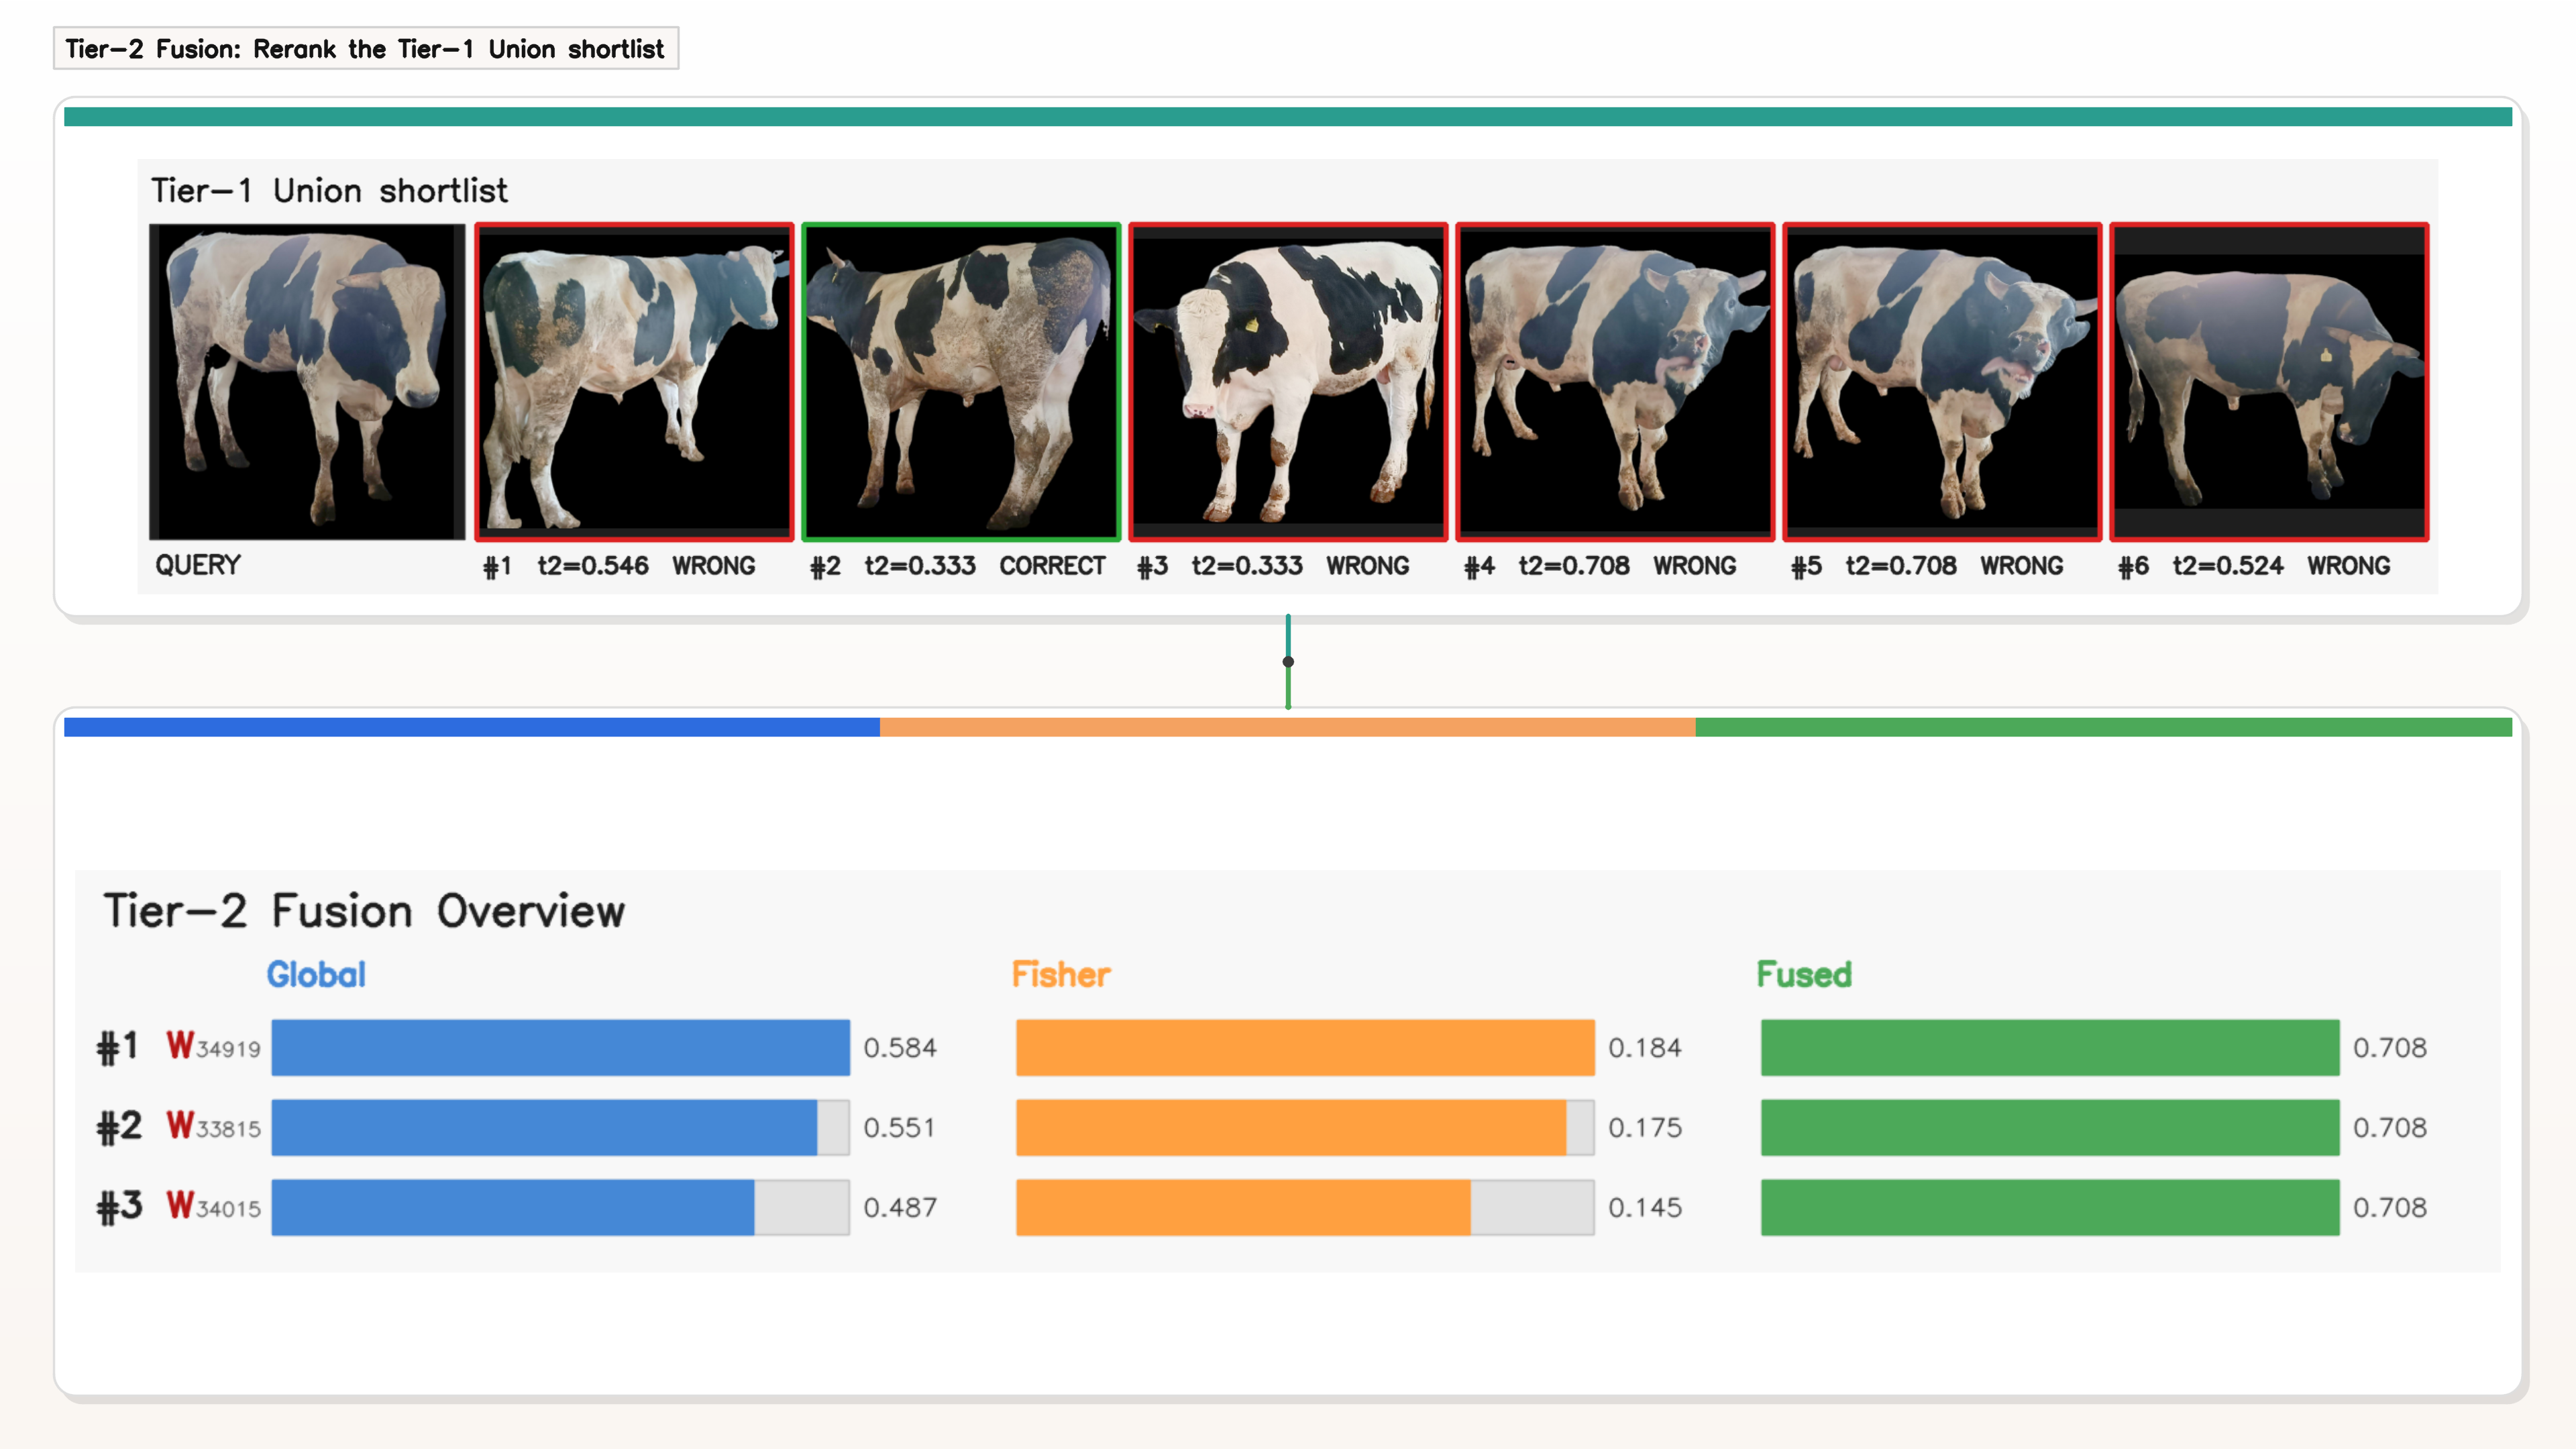
\includegraphics[width=0.98\linewidth,height=0.82\textheight,keepaspectratio]{tier2_fusion_flow.png}
\end{frame}

\begin{frame}{Tier 3: Geometric Verification (Concept)}
  \Large
  \begin{itemize}
    \item Run only on a small shortlist (most expensive stage)
    \item Match local keypoints and estimate geometric consistency (RANSAC/MAGSAC)
    \item Inlier count provides strong evidence against false matches
    \item Especially helpful on hard datasets (e.g., ELPephants)
  \end{itemize}
\end{frame}

\begin{frame}{Tier 3: Geometric Verification (Visualization)}
  \centering
  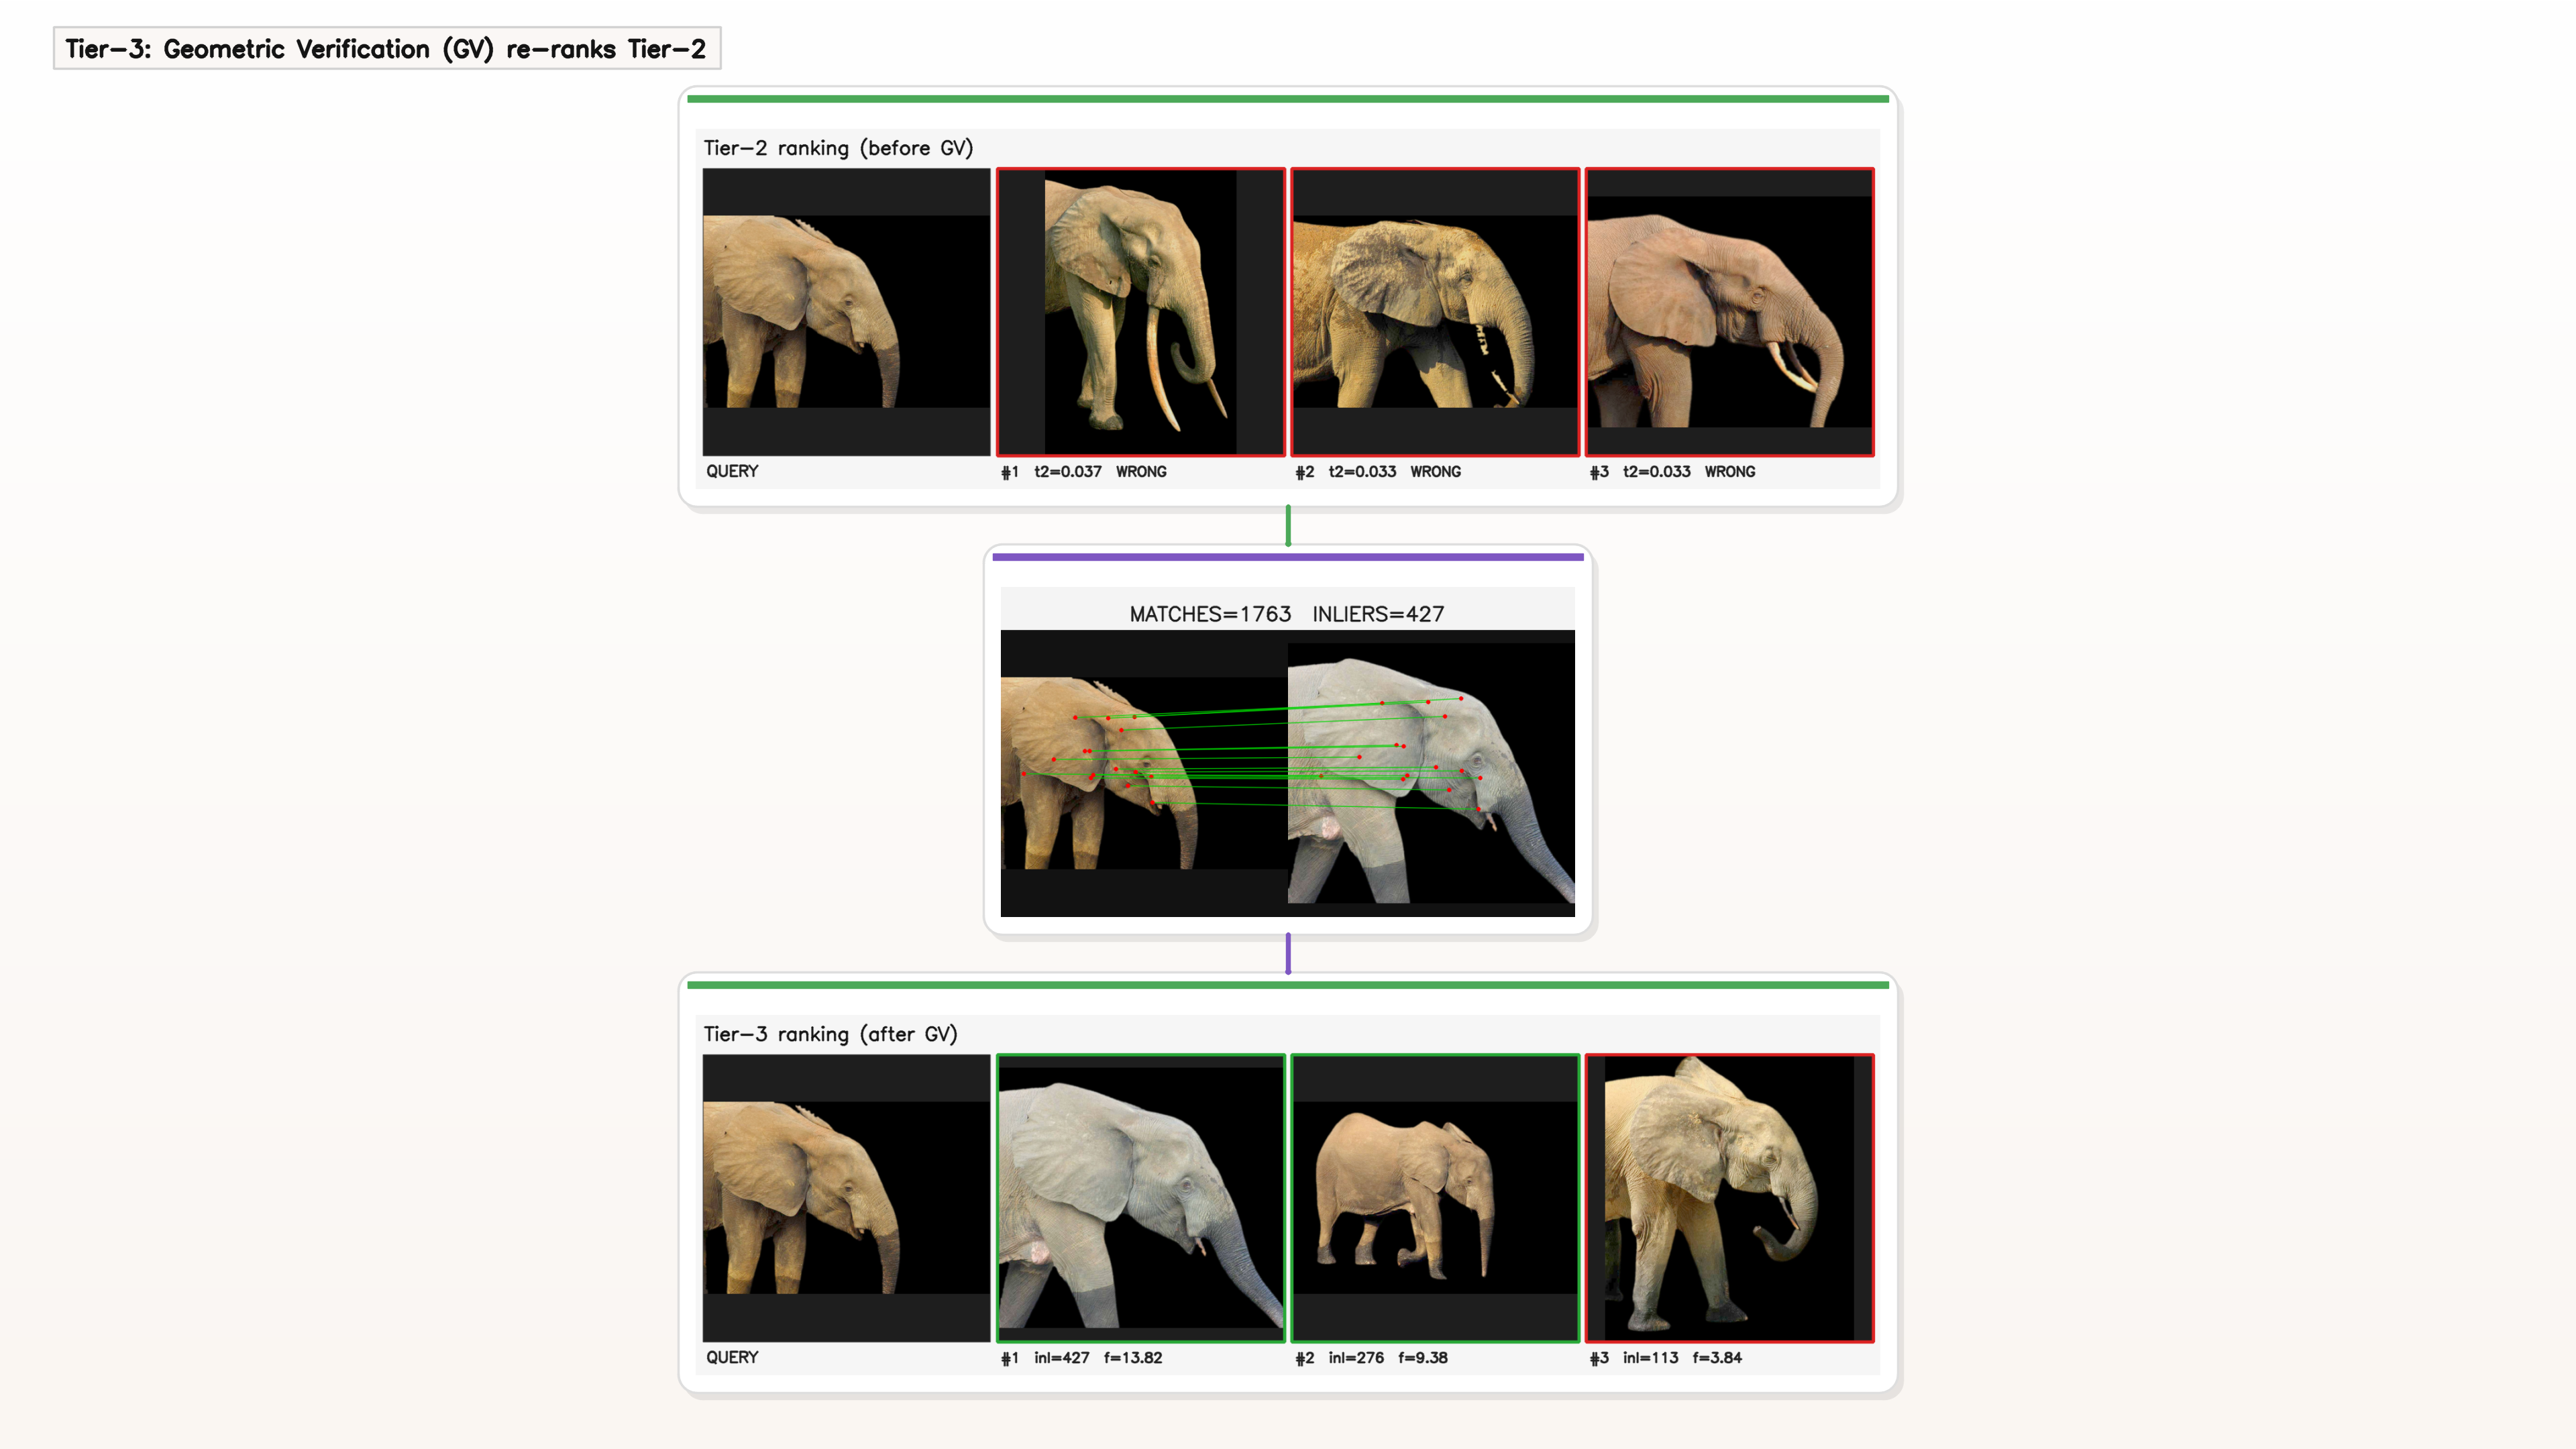
\includegraphics[width=0.98\linewidth,height=0.82\textheight,keepaspectratio]{tier3_gv_flow.png}
\end{frame}

\begin{frame}{Classification Results (Mean over 7 datasets)}
  \begin{columns}[T,totalwidth=\textwidth]
    \begin{column}{0.56\textwidth}
      \centering
      \large
      \resizebox{\linewidth}{!}{%
      \begin{tabular}{lccc}
        \toprule
        Metric & Global & WildFusion & This thesis\\
        \midrule
        Top-1 (\%) & 71.75 & \textbf{88.18} & 86.73 \\
        Top-5 (\%) & 79.58 & \textbf{91.91} & 90.70 \\
        F1 (\%) & 71.51 & \textbf{87.35} & 85.70 \\
        Runtime (min) & 0.06 & 214.52 & \textbf{42.53} \\
        \bottomrule
      \end{tabular}%
      }
    \end{column}
    \begin{column}{0.42\textwidth}
      \Large
      \begin{itemize}
        \item WildFusion is a strong calibrated fusion baseline
        \item GV is expensive $\rightarrow$ used only on a shortlist
        \item Key result: near-WildFusion accuracy at $\sim$5$\times$ lower runtime
      \end{itemize}
    \end{column}
  \end{columns}
\end{frame}

\begin{frame}{Classification Results (Selected Datasets)}
  \centering
  \scriptsize
  \setlength{\tabcolsep}{3pt}
  \renewcommand{\arraystretch}{1.10}
  \resizebox{0.98\linewidth}{!}{%
  \begin{tabular}{l l c c c c c c}
    \toprule
    Dataset & Metric & Global & WildFusion & Fisher & G+F & F+GV & G+F+GV \\
    \midrule
    ELPephants & Top-1 & 13.66 & 49.31 & 20.79 & 21.58 & 46.73 & \textbf{54.46} \\
     & Top-5 & 21.78 & 57.03 & 31.49 & 32.48 & \textbf{68.12} & 64.95 \\
     & F1 & 11.58 & 45.19 & 18.21 & 19.26 & 42.87 & \textbf{49.71} \\
    \midrule
    SealID* & Top-1 & 78.42 & \textbf{97.60} & 65.23 & 79.38 & 81.53 & 85.13 \\
     & Top-5 & 79.62 & \textbf{98.56} & 80.58 & 82.73 & 89.69 & 88.97 \\
     & F1 & 77.86 & \textbf{97.67} & 64.59 & 78.47 & 80.58 & 84.40 \\
    \midrule
    SeaStarReID2023 & Top-1 & 47.91 & \textbf{80.47} & 68.84 & 62.79 & 77.21 & 77.21 \\
     & Top-5 & 73.49 & \textbf{90.70} & 85.58 & 82.79 & 85.58 & 85.58 \\
     & F1 & 45.71 & \textbf{79.09} & 67.92 & 60.70 & 76.40 & 76.85 \\
    \bottomrule
  \end{tabular}%
  }

  \vspace{0.10cm}
  \footnotesize
  GV gain (ELPephants Top-1): 21.58 (G+F) $\rightarrow$ 54.46 (G+F+GV).
\end{frame}

\begin{frame}{ELPephants: A Stress-Test for Local + GV}
  \begin{columns}[T,totalwidth=\textwidth]
    \begin{column}{0.50\textwidth}
      \Large
      \begin{itemize}
        \item Smooth texture $\rightarrow$ weak global cues
        \item Strong pose/illumination/mud variation
        \item Local evidence + GV is crucial
        \item Best Top-1: \textbf{54.46\%} (vs 49.31\% WildFusion)
      \end{itemize}
    \end{column}
    \begin{column}{0.48\textwidth}
      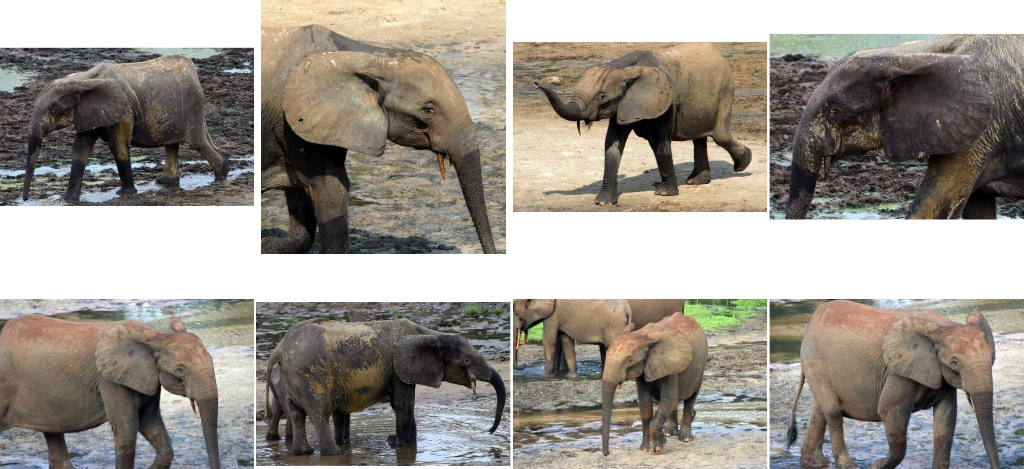
\includegraphics[width=\linewidth,height=0.80\textheight,keepaspectratio]{elephants_train_SAFE.pdf}
    \end{column}
  \end{columns}
\end{frame}

\begin{frame}{Population Counting: HITL-NIS (Idea)}
  \Large
  \begin{itemize}
    \item Goal: estimate \#individuals without full clustering
    \item Model images as clique graph $\rightarrow$ connected components
    \item Query only a small number of pairs (oracle: same/different)
    \item Use Nested Importance Sampling to reduce variance
  \end{itemize}

  \vspace{0.25cm}
  \Large
  \[
    K = \sum_{u \in V}\frac{1}{1 + d(u)}
  \]
\end{frame}

\begin{frame}{Counting Drawbacks: Human Error Matters}
  \Large
  \begin{itemize}
    \item Pair labels are highly imbalanced (mostly ``different'')
    \item False positives merge identities $\rightarrow$ underestimation collapse
    \item Confidence intervals capture sampling variance, not bias
    \item Mitigation: positive confirmation (accept ``same'' only after \(K\) consecutive votes)
  \end{itemize}
\end{frame}

\begin{frame}{Population Results (K=2): Full Table}
  \centering
  \scriptsize
  \setlength{\tabcolsep}{3pt}
  \renewcommand{\arraystretch}{1.12}
  \resizebox{0.98\linewidth}{!}{%
  \begin{tabular}{l c c c c c c c}
    \toprule
    & \textbf{ATRW} & \textbf{CowDataset} & \textbf{Chicks4FreeID} & \textbf{CZoo} & \textbf{ELPephants} & \textbf{SealID} & \textbf{SeaStarReID2023}\\
    \midrule
    \textbf{\#images} & 5415 & 1388 & 1086 & 2109 & 2078 & 2080 & 2077 \\
    \textbf{GT} & 182 & 12 & 48 & 24 & 274 & 57 & 91 \\
    \midrule
    \(p=0.00\) & \textbf{278 [132, 425]} & \textbf{12 [11, 13]} & \textbf{50 [43, 58]} & \textbf{24 [23, 26]} & \textbf{334 [267, 401]} & \textbf{56 [45, 68]} & \textbf{106 [85, 128]} \\
    \(0.02\) & \textbf{212 [124, 300]} & \textbf{13 [11, 14]} & \textbf{50 [42, 57]} & \textbf{25 [23, 27]} & \textbf{320 [259, 381]} & \textbf{65 [47, 83]} & \textbf{106 [87, 126]} \\
    \(0.05\) & \textbf{178 [116, 240]} & \textbf{13 [12, 14]} & \textbf{47 [41, 54]} & \textbf{26 [24, 27]} & 178 [157, 199] & \textbf{53 [43, 62]} & \textbf{93 [79, 106]} \\
    \(0.10\) & 72 [58, 86] & \textbf{13 [12, 14]} & 39 [34, 43] & \textbf{25 [23, 27]} & 78 [73, 83] & 45 [37, 54] & 59 [52, 66] \\
    \(0.15\) & 39 [34, 45] & \textbf{12 [11, 14]} & 27 [24, 30] & \textbf{22 [20, 24]} & 40 [38, 43] & 33 [29, 38] & 37 [33, 41] \\
    \(0.30\) & 11 [10, 12] & 8 [7, 9] & 10 [9, 11] & 13 [11, 14] & 11 [10, 12] & 13 [11, 15] & 11 [10, 12] \\
    \bottomrule
  \end{tabular}%
  }

  \vspace{0.10cm}
  \footnotesize
  \textbf{Bold}: GT falls inside the reported 95\% confidence interval.
\end{frame}

\begin{frame}{Population Results (K=1): Full Table}
  \centering
  \scriptsize
  \setlength{\tabcolsep}{3pt}
  \renewcommand{\arraystretch}{1.12}
  \resizebox{0.98\linewidth}{!}{%
  \begin{tabular}{l c c c c c c c}
    \toprule
    & \textbf{ATRW} & \textbf{CowDataset} & \textbf{Chicks4FreeID} & \textbf{CZoo} & \textbf{ELPephants} & \textbf{SealID} & \textbf{SeaStarReID2023}\\
    \midrule
    \textbf{\#images} & 5415 & 1388 & 1086 & 2109 & 2078 & 2080 & 2077 \\
    \textbf{GT} & 182 & 12 & 48 & 24 & 274 & 57 & 91 \\
    \midrule
    \(p=0.00\) & \textbf{278 [132, 425]} & \textbf{12 [11, 13]} & \textbf{50 [43, 58]} & \textbf{24 [23, 26]} & 342 [298, 386] & \textbf{56 [45, 68]} & \textbf{106 [85, 128]} \\
    \(0.02\) & 40 [33, 46] & 10 [9, 11] & 25 [22, 28] & 19 [17, 20] & 42 [41, 44] & 29 [25, 34] & 36 [32, 40] \\
    \(0.05\) & 18 [16, 20] & 8 [7, 9] & 15 [13, 16] & 13 [12, 15] & 19 [18, 20] & 17 [15, 20] & 18 [16, 20] \\
    \(0.10\) & 10 [9, 11] & 6 [5, 7] & 9 [8, 10] & 9 [8, 10] & 10 [9, 10] & 11 [9, 12] & 10 [9, 11] \\
    \(0.15\) & 7 [6, 7] & 5 [4, 5] & 6 [5, 7] & 7 [6, 8] & 7 [6, 7] & 8 [7, 8] & 7 [6, 7] \\
    \(0.30\) & 3 [3, 4] & 3 [2, 4] & 3 [3, 4] & 4 [3, 5] & 3 [3, 4] & 4 [3, 5] & 3 [3, 4] \\
    \bottomrule
  \end{tabular}%
  }

  \vspace{0.10cm}
  \footnotesize
  \textbf{Bold}: GT falls inside the reported 95\% confidence interval.
\end{frame}

\begin{frame}{Conclusions}
  \Large
  \begin{itemize}
    \item Species-agnostic 3-tier Re-ID works across multiple benchmarks
    \item Global + Fisher + GV gives strong accuracy/runtime trade-off
    \item HITL-NIS is promising, but very sensitive to human error
  \end{itemize}
\end{frame}

\begin{frame}{Future Work}
  \Large
  \begin{itemize}
    \item Validate counting with real annotators (not simulated error)
    \item Better global backbone and stronger local matching for hard datasets
    \item Link photographed-individual counts to true abundance/density
  \end{itemize}
\end{frame}

\begin{frame}[plain]
  \centering
  \vspace{0.8cm}
  {\Huge Thank you}

  \vspace{0.25cm}
  {\Large Questions?}

  \vspace{0.6cm}
  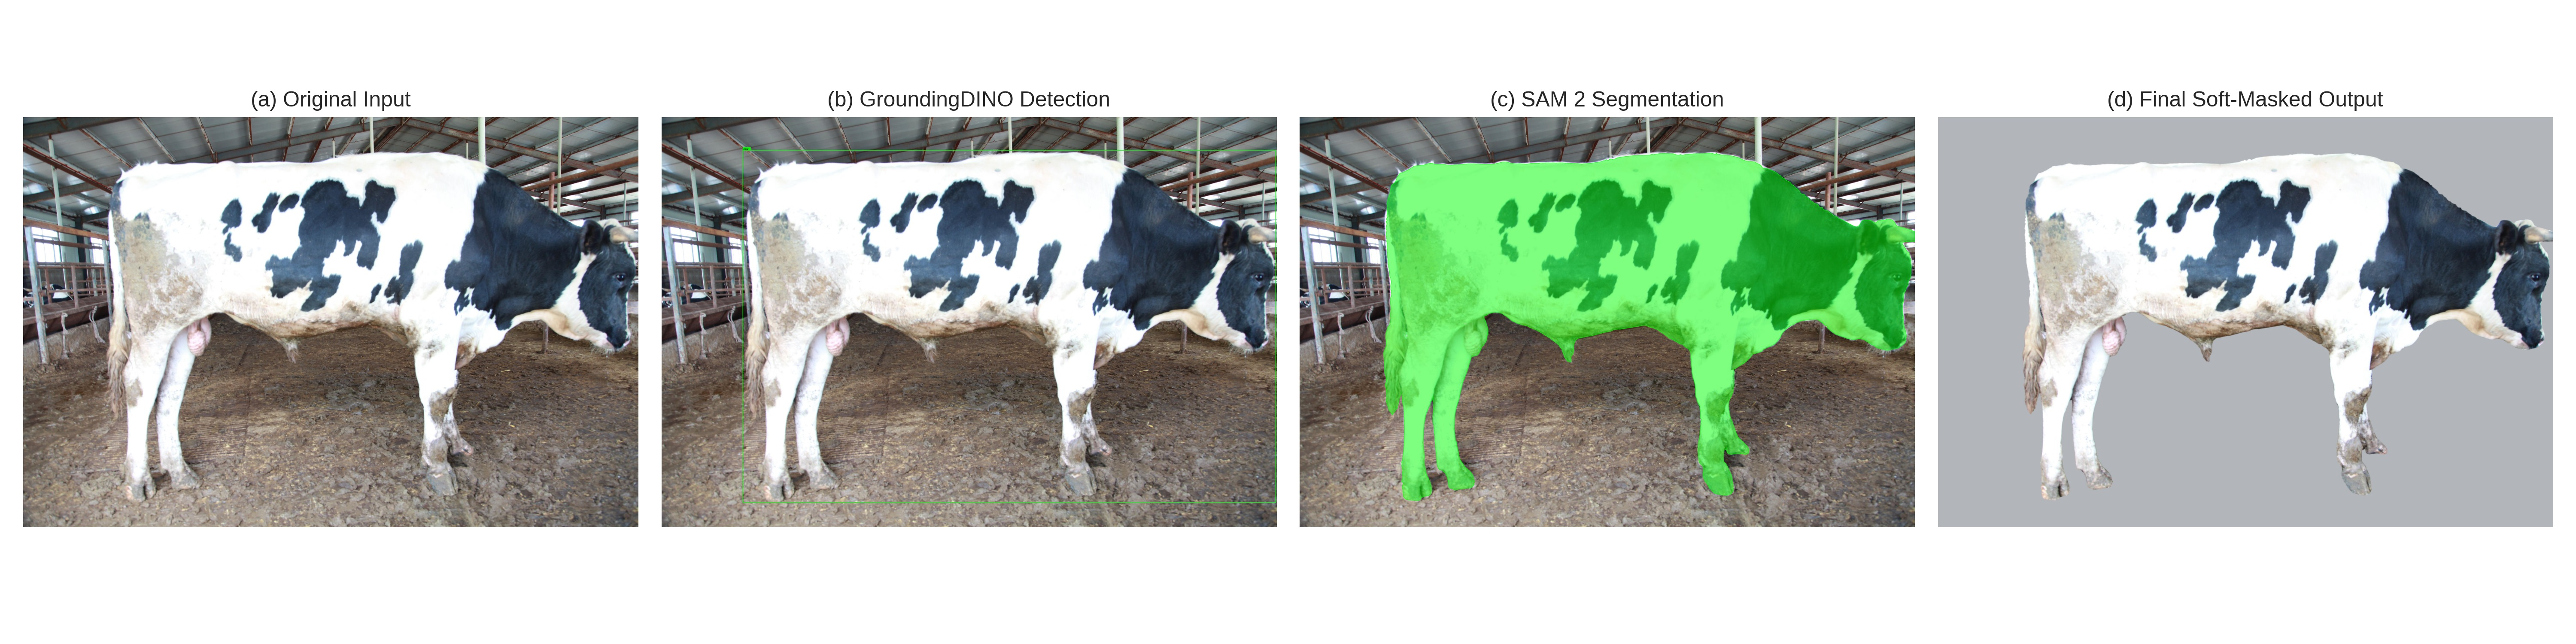
\includegraphics[width=0.78\linewidth,height=0.55\textheight,keepaspectratio]{segmentation_pipeline_vis.JPG}
\end{frame}

\end{document}
